%%%%%%%%%%%%%%%%%%%%%%%%%%%%%%%%%%%%%%%%%
% University/School Laboratory Report
% LaTeX Template
% Version 3.1 (25/3/14)
%
% This template has been downloaded from:
% http://www.LaTeXTemplates.com
%
% Original author:
% Linux and Unix Users Group at Virginia Tech Wiki 
% (https://vtluug.org/wiki/Example_LaTeX_chem_lab_report)
%
% License:
% CC BY-NC-SA 3.0 (http://creativecommons.org/licenses/by-nc-sa/3.0/)
%
%%%%%%%%%%%%%%%%%%%%%%%%%%%%%%%%%%%%%%%%%

%----------------------------------------------------------------------------------------
%	PACKAGES AND DOCUMENT CONFIGURATIONS
%----------------------------------------------------------------------------------------

\documentclass{article}

\usepackage[version=3]{mhchem} % Package for chemical equation typesetting
\usepackage{siunitx} % Provides the \SI{}{} and \si{} command for typesetting SI units
\usepackage{graphicx} % Required for the inclusion of images
\usepackage{natbib} % Required to change bibliography style to APA
\usepackage{amsmath} % Required for some math elements 

\setlength\parindent{0pt} % Removes all indentation from paragraphs

\renewcommand{\labelenumi}{\alph{enumi}.} % Make numbering in the enumerate environment by letter rather than number (e.g. section 6)

%\usepackage{times} % Uncomment to use the Times New Roman font

%----------------------------------------------------------------------------------------
%	DOCUMENT INFORMATION
%----------------------------------------------------------------------------------------

\title{Python checkers game which demonstrates machine learning} % Title

%\author{John \textsc{Smith}} % Author name

\date{\today} % Date for the report

\begin{document}

\maketitle % Insert the title, author and date

\begin{center}
%\begin{tabular}{l r}
%Date Performed: & January 1, 2012 \\ % Date the experiment was performed
%Partners: & James Smith \\ % Partner names
%& Mary Smith \\
%Instructor: & Professor Smith % Instructor/supervisor
%\end{tabular}
\end{center}

% If you wish to include an abstract, uncomment the lines below
 \begin{abstract}
 This program demonstrates a checkers program written in python in which one player learns from each game it plays. It avoids moves which result in it losing one of its pieces or ultimately lose the game. Past moves are stored in a mysql database. These are then considered before it makes a move.
% Abstract text
 \end{abstract}

%----------------------------------------------------------------------------------------
%	SECTION 1
%----------------------------------------------------------------------------------------

\section{Objective}
To demonstrate machine learning within a checkers game written in python% the atomic weight of magnesium via its reaction with oxygen and to study the stoichiometry of the reaction (as defined in \ref{definitions}):


%\begin{center}\ce{2 Mg + O2 -> 2 MgO}\end{center}

% If you have more than one objective, uncomment the below:
%\begin{description}
%\item[First Objective] \hfill \\
%Objective 1 text
%\item[Second Objective] \hfill \\
%Objective 2 text
%\end{description}

 
%----------------------------------------------------------------------------------------
%	SECTION 2
%----------------------------------------------------------------------------------------

\section{Functional Requirements}
\begin{description}
\item[Random moves for one player]
The dumb player function describes a computer player which chooses its moves entirely at random.
\item[Machine learning for player]
The smart player function describes a computer player which chooses its moves based on past experiences.
\item[Ascii Board]
The game play is displayed via a simple Ascii board. This can prove where the moves are to.
\item[Learns to win]
This program can show that smart player learns to win against the dumb player.
\end{description} 

\section{Development Methodology}
\begin{description}
%\item[Stoichiometry]
This program was developed using python 2.7. It was developed using a text editor. A link to a mysql database was used to store previous moves. It was not tested in an IDE. Some outputs were stored in a text file so the games could be manually reviewed. Print statements in addition to the board display were added so that variables could be viewed during execution.

The program was tested several times at 150 games at a time to demonstrate that the smart player was better than the dumb player.

A number of integers were adjusted to give a decent learning response. These were weights assigned to memory. A victory gave each move made by the smart player a +1 rating. A loss gave each move made by that player a -1 rating. Finally any move which resulted in the player losing a piece was given a -10 rating.

A random number generator was made to choose move with heavier ratings towards good moves was developed. However the simpler choice of choosing the best move each time was finally chosen for better results.
\end{description}
 
\section{User Interface}
\begin{description}
%\item[Stoichiometry]
In order to run one game please enter "python checkers.py".

When running you can now view the board. \\
%\\
%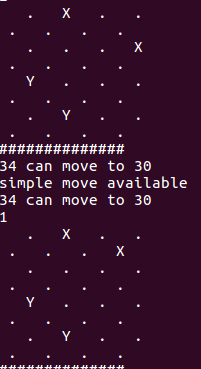
\includegraphics[width=0.65\textwidth]{Selection_002} % Include the image placeholder.png
%\\
%\begin{figure}[h]
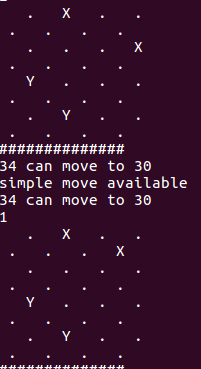
\includegraphics[width=0.5\textwidth]{Selection_002} % Include the image placeholder.png
\caption{\\Sample output of the board.}
%\end{figure}

\\ At the end of each game the winner will be displayed.



\\In order to run a batch of 150 games please enter "python trigger-mulitple.py"

You may find it necessary to redirect the output to a text file in order to review later.

The total amount of games won by each player will be stored in the mysql database.
\end{description} 
\section{Software Testing}
\begin{description}
%\item[Stoichiometry]
This program was ran through numerous times to observe the results. Bugs were spotted and removed. 
\\Occasionally the program does not exit when there is a stalemate.
The parameters were adjusted to give a more complete learning algorithm.
\end{description} 


\section{Results and Conclusions}

%The atomic weight of magnesium is concluded to be as determined by the stoichiometry of its chemical combination with oxygen. This result is in agreement with the accepted value.
This program successfully demonstrates machine learning within a python program. Checkers is quite a difficult example for this because of the sheer amount of possible combinations of pieces and moves. This makes developing a simple lookup table of all these impossible to generate within 150 games. However a subset of the lookup table can be generated to give the smart player an edge over a dumb player.


%	BIBLIOGRAPHY
%----------------------------------------------------------------------------------------

\bibliographystyle{apalike}

\bibliography{sample}

%----------------------------------------------------------------------------------------


\end{document}
